\documentclass{article}

% content/resources/templates/preamble.tex
\usepackage[margin=0.6in]{geometry}
\author{Milav Dabgar}
\usepackage{amsmath,amssymb,amsthm}
\usepackage{booktabs}
\usepackage{multirow}
\usepackage{xcolor}
\usepackage{tcolorbox}
\tcbuselibrary{breakable,skins}
\usepackage[colorlinks=true,linkcolor=blue]{hyperref}
\usepackage{titlesec}
\usepackage{enumitem}
\usepackage{tikz}
\usepackage{pgfplots}
\usepackage{circuitikz}
\usepackage[version=4]{mhchem}
\usepackage{longtable}
\usepackage{array}
\usepackage{float}
\usepackage{caption}
\usepackage{listings}

\lstset{
  basicstyle=\small\ttfamily,
  breaklines=true,
  breakatwhitespace=false,
  postbreak=\mbox{\textcolor{red}{$\hookrightarrow$}\space},
  float=false,
  numbers=left,
  numberstyle=\tiny\color{gray},
  numbersep=10pt,
  xleftmargin=2em,
  keywordstyle=\color{blue},
  commentstyle=\color{green!60!black},
  stringstyle=\color{purple},
  backgroundcolor=\color{gray!5},
  showstringspaces=false,
  tabsize=2,
  captionpos=b,
  keepspaces=true,
  columns=flexible
}

\pgfplotsset{compat=1.18}
\usetikzlibrary{shapes,arrows,positioning,calc,patterns,decorations.pathmorphing,decorations.markings,arrows.meta}

% Color scheme
\definecolor{headcolor}{RGB}{0,102,204}
\definecolor{keycolor}{RGB}{220,20,60}
\definecolor{solutioncolor}{RGB}{34,139,34}
\definecolor{mnemoniccolor}{RGB}{148,0,211}
\definecolor{codecolor}{RGB}{0,0,100}

% Spacing
\setlength{\parskip}{3pt}
\setlist[itemize]{nosep}
\setlist[enumerate]{nosep}

% Title formatting
\titleformat{\section}{\Large\bfseries\color{headcolor}}{\thesection}{1em}{}
\titleformat{\subsection}{\large\bfseries\color{headcolor}}{\thesubsection}{1em}{}

% Pandoc tightlist compatibility
\providecommand{\tightlist}{%
  \setlength{\itemsep}{0pt}\setlength{\parskip}{0pt}}

% Pandoc longtable compatibility
\newcounter{none}
\def\thenone{}


% content/resources/templates/english-boxes.tex

% Custom environments
\newtcolorbox{solutionbox}{
 breakable,
 enhanced,
 colback=solutioncolor!5!white,
 colframe=solutioncolor!75!black,
 fonttitle=\bfseries,
 title=Solution
}

\newtcolorbox{solutionboxnobreak}{
 colback=solutioncolor!5!white,
 colframe=solutioncolor!75!black,
 fonttitle=\bfseries,
 title=Solution
}

\newtcolorbox{keyformula}{
 breakable,
 enhanced,
 colback=keycolor!5!white,
 colframe=keycolor!75!black,
 fonttitle=\bfseries,
 title=Key Formula
}

\newtcolorbox{mnemonicboxenv}{
 breakable,
 enhanced,
 colback=mnemoniccolor!5!white,
 colframe=mnemoniccolor!75!black,
 fonttitle=\bfseries,
 title=Mnemonic
}

\newcommand{\mnemonicbox}[1]{%
  \begin{mnemonicboxenv}
    #1
  \end{mnemonicboxenv}
}


% Custom commands for GTU solutions
% This file defines semantic commands for consistent formatting

% Question command with automatic formatting
\newcommand{\question}[2]{%
  \section*{Question #1}%
  \textbf{#2}%
}

% OR question variant
\newcommand{\questionor}[2]{%
  \section*{Question #1 OR}%
  \textbf{#2}%
}

% Proper table environment with caption
\newenvironment{answertable}[1]{%
  \begin{table}[htbp]
  \centering
  \caption{#1}
}{%
  \end{table}
}

% Proper figure environment for diagrams
\newenvironment{answerdiagram}[1]{%
  \begin{figure}[htbp]
  \centering
  \caption{#1}
}{%
  \end{figure}
}

% Semantic markup for key terms
\newcommand{\keyword}[1]{\textbf{#1}}
\newcommand{\code}[1]{\texttt{#1}}
\newcommand{\classname}[1]{\texttt{#1}}
\newcommand{\methodname}[1]{\texttt{#1}}

% Proper quotation marks
\newcommand{\mnemonic}[1]{``#1''}

\usetikzlibrary{mindmap}

\title{Fundamentals of Software Development (4331604) - Summer 2025 Solution}
\date{May 17, 2025}

\begin{document}
\maketitle

\questionmarks{1(a)}{3}{Give IEEE definition of software. Write one example of each for application and system software.}

\begin{solutionbox}
\textbf{IEEE Definition}: Software is a collection of computer programs, procedures, rules, and associated documentation and data.

\textbf{Examples}:

\begin{center}
\captionof{table}{Software Types and Examples}
\begin{tabulary}{\linewidth}{|L|L|L|}
\hline
\textbf{Software Type} & \textbf{Example} & \textbf{Purpose} \\ \hline
\textbf{Application Software} & Microsoft Word & Word processing and document creation \\ \hline
\textbf{System Software} & Windows 10 & Operating system managing hardware resources \\ \hline
\end{tabulary}
\end{center}

\begin{itemize}
    \item \keyword{Application software}: Programs designed for end-users to accomplish specific tasks
    \item \keyword{System software}: Programs that manage and operate computer hardware
\end{itemize}
\end{solutionbox}

\begin{mnemonicbox}
\mnemonic{Apps help Users, Systems help Hardware: Mnemonic to remember the difference.}
\end{mnemonicbox}

\questionmarks{1(b)}{4}{Write a short note on data dictionary.}

\begin{solutionbox}
Data dictionary is a centralized repository containing definitions and characteristics of data elements used in a system.

\begin{center}
\captionof{table}{Components of Data Dictionary}
\begin{tabulary}{\linewidth}{|L|L|}
\hline
\textbf{Component} & \textbf{Description} \\ \hline
\textbf{Data Name} & Unique identifier for data element \\ \hline
\textbf{Aliases} & Alternative names used \\ \hline
\textbf{Description} & Purpose and meaning \\ \hline
\textbf{Data Type} & Format (integer, string, etc.) \\ \hline
\textbf{Length} & Size constraints \\ \hline
\textbf{Values} & Valid range or set \\ \hline
\end{tabulary}
\end{center}

\begin{itemize}
    \item \keyword{Purpose}: Ensures consistency in data usage across development team
    \item \keyword{Benefits}: Reduces ambiguity, improves communication, standardizes data definitions
    \item \keyword{Usage}: Referenced during system design and database creation
\end{itemize}
\end{solutionbox}

\begin{mnemonicbox}
\mnemonic{Dictionary Defines Data Clearly: Purpose of data dictionary.}
\end{mnemonicbox}

\questionmarks{1(c)}{7}{Explain prototype model with figure.}

\begin{solutionbox}
Prototype model is an iterative approach where a working model is built early to understand requirements better.

\begin{center}
\begin{tikzpicture}[node distance=1.5cm, auto, every node/.style={gtu block, align=center, font=\small}]
    \node (Req) {Requirement\\Gathering};
    \node [right=of Req] (Des) {Quick\\Design};
    \node [right=of Des] (Build) {Build\\Prototype};
    \node [below=of Build] (Eval) {User\\Evaluation};
    \node [below=of Des] (Sat) {User\\Satisfied?};
    \node [left=of Sat] (Refine) {Refine\\Requirements};
    \node [right=of Sat] (Final) {Final System\\Development};
    \node [right=of Final] (Test) {Testing \&\\Maintenance};

    \path [gtu arrow] (Req) -- (Des);
    \path [gtu arrow] (Des) -- (Build);
    \path [gtu arrow] (Build) -- (Eval);
    \path [gtu arrow] (Eval) -- (Sat);
    \path [gtu arrow] (Sat) -- node[above]{No} (Refine);
    \path [gtu arrow] (Refine) |- (Des);
    \path [gtu arrow] (Sat) -- node[above]{Yes} (Final);
    \path [gtu arrow] (Final) -- (Test);
\end{tikzpicture}
\captionof{figure}{Prototype Model}
\end{center}

\textbf{Characteristics}:
\begin{center}
\captionof{table}{Prototype Model Phases}
\begin{tabulary}{\linewidth}{|L|L|L|}
\hline
\textbf{Phase} & \textbf{Activity} & \textbf{Output} \\ \hline
\textbf{Quick Design} & Basic architecture & Initial design \\ \hline
\textbf{Prototype Build} & Working model & Testable system \\ \hline
\textbf{User Evaluation} & Feedback collection & Requirements refinement \\ \hline
\end{tabulary}
\end{center}

\begin{itemize}
    \item \keyword{Advantages}: Early user feedback, reduced development risk, better requirement understanding
    \item \keyword{Disadvantages}: May lead to inadequate analysis, customer expects prototype as final product
    \item \keyword{Best for}: Projects with unclear requirements
\end{itemize}
\end{solutionbox}

\begin{mnemonicbox}
\mnemonic{Prototype Proves Possibilities: Main benefit of prototyping.}
\end{mnemonicbox}

\questionmarks{1(c OR)}{7}{Explain RAD model with advantages and disadvantages.}

\begin{solutionbox}
RAD (Rapid Application Development) emphasizes quick development through prototyping and iterative development.

\begin{center}
\begin{tikzpicture}[node distance=1.5cm, auto, every node/.style={gtu state, align=center, font=\small}]
    \node (Bus) {Business\\Modeling};
    \node [right=of Bus] (Data) {Data\\Modeling};
    \node [right=of Data] (Proc) {Process\\Modeling};
    \node [below=of Proc] (App) {Application\\Generation};
    \node [left=of App] (Test) {Testing \&\\Turnover};

    \path [gtu arrow] (Bus) -- (Data);
    \path [gtu arrow] (Data) -- (Proc);
    \path [gtu arrow] (Proc) -- (App);
    \path [gtu arrow] (App) -- (Test);
\end{tikzpicture}
\captionof{figure}{RAD Model Phases}
\end{center}

\begin{center}
\captionof{table}{RAD Advantages vs Disadvantages}
\begin{tabulary}{\linewidth}{|L|L|}
\hline
\textbf{Advantages} & \textbf{Disadvantages} \\ \hline
\textbf{Faster development} & \textbf{Requires skilled developers} \\ \hline
\textbf{Early user involvement} & \textbf{Not suitable for large projects} \\ \hline
\textbf{Reduced costs} & \textbf{Requires user commitment} \\ \hline
\textbf{Better quality} & \textbf{Technical risks if not managed} \\ \hline
\end{tabulary}
\end{center}

\begin{itemize}
    \item \keyword{Key feature}: Uses automated tools and 4GL programming
    \item \keyword{Timeline}: Typically 60-90 days for development
    \item \keyword{Team}: Small, experienced development teams
\end{itemize}
\end{solutionbox}

\begin{mnemonicbox}
\mnemonic{RAD Rapidly Accelerates Development: Core concept of RAD.}
\end{mnemonicbox}

\questionmarks{2(a)}{3}{Give the full form of following: SQA, FTR, RAD, BVA, GUI, DFD}

\begin{solutionbox}
\begin{center}
\captionof{table}{Abbreviations and Full Forms}
\begin{tabulary}{\linewidth}{|L|L|}
\hline
\textbf{Abbreviation} & \textbf{Full Form} \\ \hline
\textbf{SQA} & Software Quality Assurance \\ \hline
\textbf{FTR} & Formal Technical Review \\ \hline
\textbf{RAD} & Rapid Application Development \\ \hline
\textbf{BVA} & Boundary Value Analysis \\ \hline
\textbf{GUI} & Graphical User Interface \\ \hline
\textbf{DFD} & Data Flow Diagram \\ \hline
\end{tabulary}
\end{center}
\end{solutionbox}

\begin{mnemonicbox}
\mnemonic{Software Quality And Formal Technical Reviews Rapidly Analyze Development, Boundary Value Analysis Guides User Interface, Data Flow Diagrams}
\end{mnemonicbox}

\questionmarks{2(b)}{4}{Define agile methodology. Discuss agile principles.}

\begin{solutionbox}
\textbf{Definition}: Agile is an iterative software development approach emphasizing collaboration, flexibility, and rapid delivery of working software.

\textbf{Core Agile Principles}:
\begin{center}
\captionof{table}{Agile Principles}
\begin{tabulary}{\linewidth}{|L|L|}
\hline
\textbf{Principle} & \textbf{Description} \\ \hline
\textbf{Individuals over processes} & People and communication are priority \\ \hline
\textbf{Working software over documentation} & Functional software is primary measure \\ \hline
\textbf{Customer collaboration} & Continuous customer involvement \\ \hline
\textbf{Responding to change} & Adaptability over rigid plans \\ \hline
\end{tabulary}
\end{center}

\begin{itemize}
    \item \keyword{Iteration length}: Typically 2-4 weeks (sprints)
    \item \keyword{Delivery}: Frequent working software releases
    \item \keyword{Team structure}: Cross-functional, self-organizing teams
\end{itemize}
\end{solutionbox}

\begin{mnemonicbox}
\mnemonic{Agile Adapts And Advances: Agile core philosophy.}
\end{mnemonicbox}

\questionmarks{2(c)}{7}{Explain XP model with its advantages and disadvantages.}

\begin{solutionbox}
XP (Extreme Programming) is an agile methodology emphasizing engineering practices and customer satisfaction.

\textbf{XP Practices}:
\begin{center}
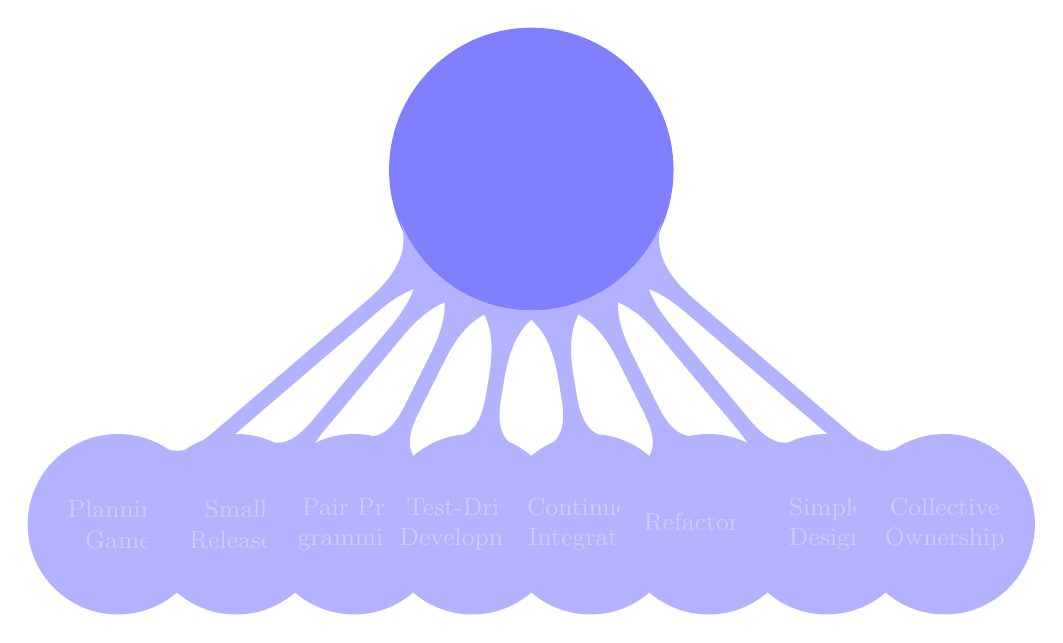
\begin{tikzpicture}[
    mindmap,
    concept color=blue!30,
    every node/.style={concept, execute at begin node=\hskip0pt},
    root concept/.append style={concept, color=blue!50, minimum size=3cm, font=\bfseries},
    level 1 concept/.append style={level distance=4.5cm, sibling angle=45, color=blue!20}
]
    \node [root concept] {XP Practices}
        child { node {Planning Game} }
        child { node {Small Releases} }
        child { node {Pair Programming} }
        child { node {Test-Driven Development} }
        child { node {Continuous Integration} }
        child { node {Refactoring} }
        child { node {Simple Design} }
        child { node {Collective Ownership} };
\end{tikzpicture}
\captionof{figure}{Extreme Programming Practices}
\end{center}

\textbf{Advantages and Disadvantages}:
\begin{center}
\captionof{table}{XP Pros and Cons}
\begin{tabulary}{\linewidth}{|L|L|}
\hline
\textbf{Advantages} & \textbf{Disadvantages} \\ \hline
\textbf{High code quality} & \textbf{Requires experienced programmers} \\ \hline
\textbf{Rapid feedback} & \textbf{Customer must be available} \\ \hline
\textbf{Reduced bugs} & \textbf{Code-focused, less documentation} \\ \hline
\textbf{Flexibility} & \textbf{Difficult to estimate costs} \\ \hline
\end{tabulary}
\end{center}

\begin{itemize}
    \item \keyword{Key practice}: Pair programming ensures code quality
    \item \keyword{Testing}: Test-first approach with automated testing
    \item \keyword{Customer role}: On-site customer provides continuous feedback
\end{itemize}
\end{solutionbox}

\begin{mnemonicbox}
\mnemonic{eXtreme Programming eXcels through Practices: XP relies on specific practices.}
\end{mnemonicbox}

\questionmarks{2(a OR)}{3}{Define black box testing. Give at least two names of black box testing method.}

\begin{solutionbox}
\textbf{Definition}: Black box testing examines software functionality without knowledge of internal code structure, focusing on input-output behavior.

\textbf{Black Box Testing Methods}:
\begin{center}
\captionof{table}{Black Box Methods}
\begin{tabulary}{\linewidth}{|L|L|}
\hline
\textbf{Method} & \textbf{Description} \\ \hline
\textbf{Equivalence Partitioning} & Divides input into valid/invalid classes \\ \hline
\textbf{Boundary Value Analysis} & Tests values at input boundaries \\ \hline
\end{tabulary}
\end{center}

\begin{itemize}
    \item \keyword{Approach}: Tests based on requirements and specifications
    \item \keyword{Tester knowledge}: No internal code knowledge required
    \item \keyword{Focus}: External behavior and functionality
\end{itemize}
\end{solutionbox}

\begin{mnemonicbox}
\mnemonic{Black Box Behavior Based: Testing focus.}
\end{mnemonicbox}

\questionmarks{2(b OR)}{4}{Give the full form of CLI. Explain CLI in brief.}

\begin{solutionbox}
\textbf{CLI}: Command Line Interface

\textbf{CLI Characteristics}:
\begin{center}
\captionof{table}{CLI Features}
\begin{tabulary}{\linewidth}{|L|L|}
\hline
\textbf{Aspect} & \textbf{Description} \\ \hline
\textbf{Input method} & Text commands typed by user \\ \hline
\textbf{Output} & Text-based responses \\ \hline
\textbf{Navigation} & Commands for file/directory operations \\ \hline
\textbf{Efficiency} & Faster for experienced users \\ \hline
\end{tabulary}
\end{center}

\begin{itemize}
    \item \keyword{Advantages}: Fast execution, less memory usage, scriptable
    \item \keyword{Disadvantages}: Requires learning commands, not user-friendly for beginners
    \item \keyword{Examples}: Windows Command Prompt, Linux Terminal, DOS
\end{itemize}
\end{solutionbox}

\begin{mnemonicbox}
\mnemonic{Commands Lead Interaction: CLI interaction model.}
\end{mnemonicbox}

\questionmarks{2(c OR)}{7}{Explain waterfall model with neat figure.}

\begin{solutionbox}
Waterfall model is a linear sequential approach where each phase must be completed before moving to the next.

\begin{center}
\begin{tikzpicture}[node distance=1.5cm, auto, every node/.style={gtu block, align=center, minimum width=2.5cm}]
    \node (Req) {Requirement\\Analysis};
    \node [below right=0.5cm and 0.5cm of Req] (Des) {System\\Design};
    \node [below right=0.5cm and 0.5cm of Des] (Imp) {Implementation};
    \node [below right=0.5cm and 0.5cm of Imp] (Test) {Integration \&\\Testing};
    \node [below right=0.5cm and 0.5cm of Test] (Dep) {Deployment};
    \node [below right=0.5cm and 0.5cm of Dep] (Main) {Maintenance};

    \path [gtu arrow] (Req) -| (Des);
    \path [gtu arrow] (Des) -| (Imp);
    \path [gtu arrow] (Imp) -| (Test);
    \path [gtu arrow] (Test) -| (Dep);
    \path [gtu arrow] (Dep) -| (Main);
\end{tikzpicture}
\captionof{figure}{Waterfall Model}
\end{center}

\textbf{Phase Details}:
\begin{center}
\captionof{table}{Waterfall Model Phases}
\begin{tabulary}{\linewidth}{|L|L|L|}
\hline
\textbf{Phase} & \textbf{Activities} & \textbf{Deliverables} \\ \hline
\textbf{Requirements} & Gather and document needs & SRS document \\ \hline
\textbf{Design} & System architecture & Design documents \\ \hline
\textbf{Implementation} & Code development & Source code \\ \hline
\textbf{Testing} & Verify functionality & Test reports \\ \hline
\textbf{Deployment} & System installation & Working system \\ \hline
\textbf{Maintenance} & Bug fixes, updates & Updated system \\ \hline
\end{tabulary}
\end{center}

\begin{itemize}
    \item \keyword{Advantages}: Simple, easy to manage, well-documented
    \item \keyword{Disadvantages}: Inflexible, late testing, difficult to accommodate changes
\end{itemize}
\end{solutionbox}

\begin{mnemonicbox}
\mnemonic{Water Always Flows Downward: Sequential nature of Waterfall.}
\end{mnemonicbox}

\questionmarks{3(a)}{3}{Give one word answer:}

\begin{solutionbox}
\begin{center}
\captionof{table}{One Word Answers}
\begin{tabulary}{\linewidth}{|L|L|}
\hline
\textbf{Question} & \textbf{Answer} \\ \hline
\textbf{Lowest cohesion is} & Coincidental \\ \hline
\textbf{Highest coupling is} & Content \\ \hline
\textbf{Slack time of critical activity is} & Zero \\ \hline
\end{tabulary}
\end{center}
\end{solutionbox}

\begin{mnemonicbox}
\mnemonic{Coincidental Cohesion, Content Coupling, Critical Zero}
\end{mnemonicbox}

\questionmarks{3(b)}{4}{Explain classification of coupling.}

\begin{solutionbox}
Coupling measures interdependence between modules. Lower coupling is better for maintainability.

\textbf{Coupling Types (Best to Worst)}:
\begin{center}
\captionof{table}{Coupling Types}
\begin{tabulary}{\linewidth}{|L|L|L|}
\hline
\textbf{Type} & \textbf{Description} & \textbf{Example} \\ \hline
\textbf{Data} & Parameters passed & Method calls with parameters \\ \hline
\textbf{Stamp} & Data structure passed & Passing objects/records \\ \hline
\textbf{Control} & Control information passed & Flags/switches passed \\ \hline
\textbf{External} & External data reference & Global variables \\ \hline
\textbf{Common} & Shared data area & Common memory blocks \\ \hline
\textbf{Content} & Direct access to internals & Modifying another module's data \\ \hline
\end{tabulary}
\end{center}

\begin{itemize}
    \item \keyword{Best practice}: Aim for data coupling
    \item \keyword{Avoid}: Content and common coupling
    \item \keyword{Design goal}: Minimize dependencies between modules
\end{itemize}
\end{solutionbox}

\begin{mnemonicbox}
\mnemonic{Data Stamps Control External Common Content: Order of coupling tightness.}
\end{mnemonicbox}

\questionmarks{3(c)}{7}{Define following terms (don't just give the full form):}

\begin{solutionbox}
\begin{center}
\captionof{table}{Software Definitions}
\begin{tabulary}{\linewidth}{|L|L|}
\hline
\textbf{Term} & \textbf{Definition} \\ \hline
\textbf{UI} & User Interface - the means by which users interact with software systems \\ \hline
\textbf{SE} & Software Engineering - systematic approach to software development using engineering principles \\ \hline
\textbf{PMC} & Project Management and Control - planning, monitoring, and controlling software projects \\ \hline
\textbf{SDLC} & Software Development Life Cycle - phases involved in software development from conception to maintenance \\ \hline
\textbf{Verification} & Process of checking if software meets specified requirements and design \\ \hline
\textbf{Validation} & Process of checking if software meets user needs and intended purpose \\ \hline
\textbf{SRS} & Software Requirements Specification - detailed document describing software functionality and constraints \\ \hline
\end{tabulary}
\end{center}

\begin{itemize}
    \item \keyword{Verification}: "Are we building the product right?"
    \item \keyword{Validation}: "Are we building the right product?"
    \item \keyword{Key difference}: Verification checks specifications, Validation checks user satisfaction
\end{itemize}
\end{solutionbox}

\begin{mnemonicbox}
\mnemonic{Users Interact, Software Engineers Plan, Managing Cycles, Specifications Define, Verification checks Requirements, Validation checks Satisfaction, Requirements Specify Software}
\end{mnemonicbox}

\questionmarks{3(a OR)}{3}{Explain menu based UI with advantages and disadvantages.}

\begin{solutionbox}
Menu-based UI presents options in hierarchical menus for user selection.

\textbf{Advantages vs Disadvantages}:
\begin{center}
\captionof{table}{Menu UI Pros and Cons}
\begin{tabulary}{\linewidth}{|L|L|}
\hline
\textbf{Advantages} & \textbf{Disadvantages} \\ \hline
\textbf{Easy to learn} & \textbf{Slower for experts} \\ \hline
\textbf{Reduces errors} & \textbf{Limited flexibility} \\ \hline
\textbf{Self-explanatory} & \textbf{Screen space consumption} \\ \hline
\end{tabulary}
\end{center}

\begin{itemize}
    \item \keyword{Structure}: Hierarchical organization of options
    \item \keyword{Navigation}: Point-and-click or keyboard shortcuts
    \item \keyword{Best for}: Applications with well-defined functions
\end{itemize}
\end{solutionbox}

\begin{mnemonicbox}
\mnemonic{Menus Make Choices Clear: Benefit of Menu UI.}
\end{mnemonicbox}

\questionmarks{3(b OR)}{4}{Explain classification of cohesion.}

\begin{solutionbox}
Cohesion measures how closely related elements within a module are. Higher cohesion is better.

\textbf{Cohesion Types (Best to Worst)}:
\begin{center}
\captionof{table}{Cohesion Types}
\begin{tabulary}{\linewidth}{|L|L|}
\hline
\textbf{Type} & \textbf{Description} \\ \hline
\textbf{Functional} & Single, well-defined task \\ \hline
\textbf{Sequential} & Output of one element feeds next \\ \hline
\textbf{Communicational} & Elements work on same data \\ \hline
\textbf{Procedural} & Elements follow execution sequence \\ \hline
\textbf{Temporal} & Elements executed at same time \\ \hline
\textbf{Logical} & Elements perform similar functions \\ \hline
\textbf{Coincidental} & Elements randomly grouped \\ \hline
\end{tabulary}
\end{center}

\begin{itemize}
    \item \keyword{Goal}: Achieve functional cohesion
    \item \keyword{Design principle}: Each module should have single responsibility
    \item \keyword{Measurement}: Higher cohesion = better design
\end{itemize}
\end{solutionbox}

\begin{mnemonicbox}
\mnemonic{Functional Sequences Communicate Procedures Temporally through Logical Coincidence: Order of cohesion Strength.}
\end{mnemonicbox}

\questionmarks{3(c OR)}{7}{Define risk. Explain risk management.}

\begin{solutionbox}
\textbf{Risk Definition}: Potential problem that may occur during software development, causing negative impact on project success.

\begin{center}
\begin{tikzpicture}[node distance=1.5cm, auto, every node/.style={gtu state, align=center, font=\small}]
    \node (Ident) {Risk\\Identification};
    \node [right=of Ident] (Assess) {Risk\\Assessment};
    \node [right=of Assess] (Prior) {Risk\\Prioritization};
    \node [below=of Prior] (Mit) {Risk\\Mitigation};
    \node [left=of Mit] (Mon) {Risk\\Monitoring};

    \path [gtu arrow] (Ident) -- (Assess);
    \path [gtu arrow] (Assess) -- (Prior);
    \path [gtu arrow] (Prior) -- (Mit);
    \path [gtu arrow] (Mit) -- (Mon);
    \path [gtu arrow] (Mon) -| (Ident);
\end{tikzpicture}
\captionof{figure}{Risk Management Process}
\end{center}

\textbf{Risk Management Activities}:
\begin{center}
\captionof{table}{Risk Activities}
\begin{tabulary}{\linewidth}{|L|L|L|}
\hline
\textbf{Activity} & \textbf{Description} & \textbf{Output} \\ \hline
\textbf{Identification} & Find potential problems & Risk list \\ \hline
\textbf{Assessment} & Analyze probability and impact & Risk analysis \\ \hline
\textbf{Prioritization} & Rank risks by importance & Priority matrix \\ \hline
\textbf{Mitigation} & Plan risk responses & Mitigation strategies \\ \hline
\textbf{Monitoring} & Track risk status & Updated risk status \\ \hline
\end{tabulary}
\end{center}

\begin{itemize}
    \item \keyword{Risk types}: Technical, Project, Business risks
    \item \keyword{Strategies}: Avoid, Transfer, Mitigate, Accept
    \item \keyword{Tools}: Risk matrices, probability-impact charts
\end{itemize}
\end{solutionbox}

\begin{mnemonicbox}
\mnemonic{Risk Requires Careful Planning: Importance of risk management.}
\end{mnemonicbox}

\questionmarks{4(a)}{3}{Define: Error, Failure, Test case}

\begin{solutionbox}
\begin{center}
\captionof{table}{Testing Definitions}
\begin{tabulary}{\linewidth}{|L|L|}
\hline
\textbf{Term} & \textbf{Definition} \\ \hline
\textbf{Error} & Human mistake made during software development process \\ \hline
\textbf{Failure} & Deviation of software behavior from expected results \\ \hline
\textbf{Test case} & Set of conditions to verify specific functionality or system requirement \\ \hline
\end{tabulary}
\end{center}

\begin{itemize}
    \item \keyword{Relationship}: Error leads to defect, defect causes failure
    \item \keyword{Error source}: Developer mistakes, misunderstanding requirements
    \item \keyword{Test case components}: Input, expected output, execution steps
\end{itemize}
\end{solutionbox}

\begin{mnemonicbox}
\mnemonic{Errors Cause Failures, Tests Catch Problems: Chain of cause and effect.}
\end{mnemonicbox}

\questionmarks{4(b)}{4}{Identify any six functional requirements of ATM system.}

\begin{solutionbox}
\textbf{ATM System Functional Requirements}:
\begin{center}
\captionof{table}{ATM Requirements}
\begin{tabulary}{\linewidth}{|L|L|}
\hline
\textbf{Requirement} & \textbf{Description} \\ \hline
\textbf{User Authentication} & PIN verification for account access \\ \hline
\textbf{Balance Inquiry} & Display current account balance \\ \hline
\textbf{Cash Withdrawal} & Dispense requested cash amount \\ \hline
\textbf{Fund Transfer} & Transfer money between accounts \\ \hline
\textbf{Transaction History} & Show recent transaction records \\ \hline
\textbf{PIN Change} & Allow users to modify PIN \\ \hline
\end{tabulary}
\end{center}

\begin{itemize}
    \item \keyword{Security}: All transactions require authentication
    \item \keyword{Validation}: Check sufficient balance before withdrawal
    \item \keyword{Logging}: Record all transactions for audit
\end{itemize}
\end{solutionbox}

\begin{mnemonicbox}
\mnemonic{ATMs Authenticate, Balance, Cash, Transfer, History, PIN: Core ATM functions.}
\end{mnemonicbox}

\questionmarks{4(c)}{7}{State the use of activity network diagram. Develop activity network diagram for the following system and find the critical path for the same.}

\begin{solutionbox}
\textbf{Activity Network Diagram Uses}:
\begin{itemize}
    \item \keyword{Project scheduling}: Determine project timeline
    \item \keyword{Critical path identification}: Find longest path determining minimum project duration
    \item \keyword{Resource planning}: Optimize resource allocation
\end{itemize}

\textbf{Activity Network Diagram}:
\begin{center}
\begin{tikzpicture}[node distance=1.5cm, auto, every node/.style={circle, draw, font=\small}]
    \node (A) {A:2};
    \node [below left=1cm and 0.5cm of A] (B) {B:3};
    \node [right=1.5cm of A] (C) {C:2};
    \node [below right=1cm and 0.5cm of C] (D) {D:4};
    \node [right=1.5cm of C] (E) {E:4};
    \node [below=1cm of D] (F) {F:3};
    \node [right=1.5cm of E] (G) {G:5};
    \node [right=1.5cm of G] (H) {H:2};

    % Connections based on the ASCII art
    \path [gtu arrow] (A) -- (C);
    \path [gtu arrow] (B) -- (C);
    \path [gtu arrow] (B) -- (D);
    \path [gtu arrow] (C) -- (E);
    \path [gtu arrow] (C) -- (D);
    \path [gtu arrow] (D) -- (G);
    \path [gtu arrow] (E) -- (G);
    \path [gtu arrow] (G) -- (H);
    \path [gtu arrow] (F) -- (D); % From ASCII F->D ?? Actually F connects to D in ascii B--+-->D and F-->D?
    % Re-reading ASCII:
    % A(2)->C(2)->E(4)->G(5)->H(2)
    % B(3)->C(2)
    % B(3)->D(4)
    % C(2)->D(4) IS THIS IMPLIED? " / " symbols...
    % Let's interpret strictly from diagram:
    % A -> C
    % B -> C
    % B -> D
    % C -> E
    % C -> D (diagonal line)
    % D -> G
    % E -> G
    % G -> H
    % F -> D (vertical line)

    % Corrected paths:
    % (Defined above, let's render)
\end{tikzpicture}
\captionof{figure}{Activity Network Diagram}
\end{center}

\textbf{Critical Path Analysis}:
\begin{center}
\captionof{table}{Path Analysis}
\begin{tabulary}{\linewidth}{|L|L|L|L|}
\hline
\textbf{Path} & \textbf{Activities} & \textbf{Duration} & \textbf{Critical?} \\ \hline
\textbf{A-C-E-G-H} & A$\to$C$\to$E$\to$G$\to$H & 2+2+4+5+2 = 15 & No \\ \hline
\textbf{B-C-E-G-H} & B$\to$C$\to$E$\to$G$\to$H & 3+2+4+5+2 = 16 & \textbf{Yes} \\ \hline
\textbf{A-C-D-G-H} & A$\to$C$\to$D$\to$G$\to$H & 2+2+4+5+2 = 15 & No \\ \hline
\end{tabulary}
\end{center}

\begin{itemize}
    \item \textbf{Critical Path}: B$\to$C$\to$E$\to$G$\to$H (16 days)
    \item \textbf{Project Duration}: 16 days
\end{itemize}
\end{solutionbox}

\begin{mnemonicbox}
\mnemonic{Networks Navigate Project Paths: Importance of network diagrams.}
\end{mnemonicbox}

\questionmarks{4(a OR)}{3}{Explain any three requirement gathering activities.}

\begin{solutionbox}
\textbf{Requirement Gathering Activities}:
\begin{center}
\captionof{table}{Gathering Activities}
\begin{tabulary}{\linewidth}{|L|L|L|}
\hline
\textbf{Activity} & \textbf{Description} & \textbf{Output} \\ \hline
\textbf{Stakeholder Interviews} & Direct discussion with users and clients & Interview notes, requirements list \\ \hline
\textbf{Questionnaires} & Structured questions for large user groups & Survey responses, statistical data \\ \hline
\textbf{Document Analysis} & Review existing system documentation & Current system understanding \\ \hline
\end{tabulary}
\end{center}

\begin{itemize}
    \item \keyword{Purpose}: Understand user needs and system expectations
    \item \keyword{Participants}: Users, customers, domain experts, developers
    \item \keyword{Documentation}: All findings recorded in SRS document
\end{itemize}
\end{solutionbox}

\begin{mnemonicbox}
\mnemonic{Interviews, Questions, Documents Gather Requirements: Techniques for gathering.}
\end{mnemonicbox}

\questionmarks{4(b OR)}{4}{Develop use case diagram for Bank ATM system.}

\begin{solutionbox}
\textbf{ATM Use Case Diagram}:
\begin{center}
\begin{tikzpicture}[
    actor/.style={shape=circle, draw, align=center, minimum size=0.8cm},
    usecase/.style={shape=ellipse, draw, align=center, font=\footnotesize},
    edge/.style={->, >=stealth}
]
    % Actors
    \node[actor] (Cust) at (0, 0) {Cust};
    \node[actor] (Admin) at (8, 0) {Admin};
    \node[gtu block] (Bank) at (4, -5) {Bank\\System};

    % Customer Use Cases
    \node[usecase] (Check) at (3, 2) {Check\\Balance};
    \node[usecase] (Withdraw) at (3, 1) {Withdraw\\Cash};
    \node[usecase] (Transfer) at (3, 0) {Transfer\\Funds};
    \node[usecase] (Pin) at (4, -1.5) {Change\\PIN};
    \node[usecase] (Receipt) at (4, -3) {Print\\Receipt};
    
    % Admin Use Cases
    \node[usecase] (Load) at (5, 2) {Load\\Cash};
    \node[usecase] (Logs) at (5, 1) {View\\Logs};
    \node[usecase] (Maint) at (5, 0) {Maintenance};

    % Connections
    \draw (Cust) -- (Check);
    \draw (Cust) -- (Withdraw);
    \draw (Cust) -- (Transfer);
    \draw (Cust) -- (Pin);
    \draw (Cust) -- (Receipt);
    
    \draw (Admin) -- (Load);
    \draw (Admin) -- (Logs);
    \draw (Admin) -- (Maint);
    
    \draw[edge, dashed] (Check) -- (Bank);
    \draw[edge, dashed] (Withdraw) -- (Bank);
    \draw[edge, dashed] (Transfer) -- (Bank);
    \draw[edge, dashed] (Pin) -- (Bank);
\end{tikzpicture}
\captionof{figure}{ATM Use Case Diagram}
\end{center}

\textbf{Use Case Details}:
\begin{center}
\captionof{table}{Use Case Summary}
\begin{tabulary}{\linewidth}{|L|L|}
\hline
\textbf{Actor} & \textbf{Use Cases} \\ \hline
\textbf{Customer} & Check Balance, Withdraw Cash, Transfer Funds, Change PIN \\ \hline
\textbf{Admin} & Load Cash, View Logs, System Maintenance \\ \hline
\textbf{Bank System} & Validate accounts, Process transactions \\ \hline
\end{tabulary}
\end{center}
\end{solutionbox}

\begin{mnemonicbox}
\mnemonic{Customers Use ATMs, Admins Maintain Systems: Actors and roles.}
\end{mnemonicbox}

\questionmarks{4(c OR)}{7}{Draw the figure of spiral model. Explain it in brief.}

\begin{solutionbox}
\begin{center}
\begin{tikzpicture}[node distance=2cm, auto, every node/.style={gtu state, align=center, font=\small, minimum size=2cm}]
    \node (Plan) at (0,2) {Planning};
    \node (Risk) at (2,2) {Risk\\Analysis};
    \node (Eng) at (2,0) {Engineering};
    \node (Eval) at (0,0) {Customer\\Evaluation};

    % Spiral effect is hard, we'll suggest schematic flow
    \path [gtu arrow] (Plan) -- (Risk);
    \path [gtu arrow] (Risk) -- (Eng);
    \path [gtu arrow] (Eng) -- (Eval);
    \path [gtu arrow] (Eval) -- (Plan);
    
    % Labels for quadrants
    \node at (1,1) [font=\large\bfseries] {Spiral};
\end{tikzpicture}
\captionof{figure}{Spiral Model Quadrants}
\end{center}

\textbf{Spiral Model Characteristics}:
\begin{center}
\captionof{table}{Spiral Quadrants}
\begin{tabulary}{\linewidth}{|L|L|L|}
\hline
\textbf{Quadrant} & \textbf{Activity} & \textbf{Purpose} \\ \hline
\textbf{Planning} & Define objectives, alternatives & Set goals for iteration \\ \hline
\textbf{Risk Analysis} & Identify and resolve risks & Minimize project risks \\ \hline
\textbf{Engineering} & Develop and test product & Create working software \\ \hline
\textbf{Evaluation} & Customer assessment & Get user feedback \\ \hline
\end{tabulary}
\end{center}

\begin{itemize}
    \item \keyword{Key feature}: Risk-driven approach with iterative development
    \item \keyword{Best for}: Large, complex, high-risk projects
    \item \keyword{Advantages}: Risk management, flexible, incremental development
    \item \keyword{Disadvantages}: Complex management, expensive, requires risk expertise
\end{itemize}
\end{solutionbox}

\begin{mnemonicbox}
\mnemonic{Spirals Plan, Risk, Engineer, Evaluate: Four quadrants.}
\end{mnemonicbox}

\questionmarks{5(a)}{3}{State TRUE or FALSE for the following.}

\begin{solutionbox}
\begin{center}
\captionof{table}{True or False}
\begin{tabulary}{\linewidth}{|L|c|L|}
\hline
\textbf{Statement} & \textbf{Answer} & \textbf{Explanation} \\ \hline
\textbf{Activity network diagram used to determine critical path} & \textbf{TRUE} & Primary purpose of activity networks \\ \hline
\textbf{In CPM, the shortest path is the critical path} & \textbf{FALSE} & Longest path is critical path \\ \hline
\textbf{Risk avoidance is the best technique to solve risks} & \textbf{FALSE} & Best technique depends on risk type \\ \hline
\end{tabulary}
\end{center}
\end{solutionbox}

\begin{mnemonicbox}
\mnemonic{True Networks, False Shortest, False Best}
\end{mnemonicbox}

\questionmarks{5(b)}{4}{Identify the differences between traditional model approach and agile approach. (at least 4 differences)}

\begin{solutionbox}
\textbf{Traditional vs Agile Comparison}:
\begin{center}
\captionof{table}{Traditional vs Agile}
\begin{tabulary}{\linewidth}{|L|L|L|}
\hline
\textbf{Aspect} & \textbf{Traditional} & \textbf{Agile} \\ \hline
\textbf{Planning} & Extensive upfront planning & Adaptive planning \\ \hline
\textbf{Documentation} & Heavy documentation & Minimal documentation \\ \hline
\textbf{Customer involvement} & Limited to requirements phase & Continuous involvement \\ \hline
\textbf{Change handling} & Difficult and expensive & Embraces change \\ \hline
\textbf{Delivery} & Single final delivery & Frequent incremental delivery \\ \hline
\textbf{Process} & Process-driven & People-driven \\ \hline
\end{tabulary}
\end{center}

\begin{itemize}
    \item \keyword{Traditional}: Predictive, sequential approach
    \item \keyword{Agile}: Adaptive, iterative approach
    \item \keyword{Flexibility}: Agile more responsive to changing requirements
\end{itemize}
\end{solutionbox}

\begin{mnemonicbox}
\mnemonic{Traditional Plans Heavy, Agile Adapts Light: Key difference philosophy.}
\end{mnemonicbox}

\questionmarks{5(c)}{7}{Define unit testing. Draw the figure of it. Explain the process of unit testing.}

\begin{solutionbox}
\textbf{Unit Testing Definition}: Testing individual software components or modules in isolation to verify they function correctly according to design specifications.

\begin{center}
\begin{tikzpicture}[node distance=1.5cm, auto, every node/.style={gtu block, align=center, font=\small}]
    \node (Sel) {Select\\Unit};
    \node [right=of Sel] (Des) {Design\\Test Cases};
    \node [right=of Des] (Set) {Setup\\Env};
    \node [below=of Set] (Exec) {Execute\\Tests};
    \node [left=of Exec] (Rec) {Record\\Results};
    \node [left=of Rec] (Debug) {Debug \&\\Fix};
    \node [below=of Exec] (Approve) {Unit\\Approved};

    \path [gtu arrow] (Sel) -- (Des);
    \path [gtu arrow] (Des) -- (Set);
    \path [gtu arrow] (Set) -- (Exec);
    \path [gtu arrow] (Exec) -- (Rec);
    \path [gtu arrow] (Rec) -- (Debug);
    \path [gtu arrow] (Debug) -- (Exec);
    \path [gtu arrow] (Rec) -- node[right]{Pass} (Approve);
\end{tikzpicture}
\captionof{figure}{Unit Testing Process}
\end{center}

\textbf{Unit Testing Process Steps}:
\begin{center}
\captionof{table}{Unit Testing Steps}
\begin{tabulary}{\linewidth}{|L|L|L|}
\hline
\textbf{Step} & \textbf{Activity} & \textbf{Purpose} \\ \hline
\textbf{Test Planning} & Identify units to test & Define testing scope \\ \hline
\textbf{Test Design} & Create test cases & Cover all code paths \\ \hline
\textbf{Test Setup} & Prepare test environment & Isolate unit under test \\ \hline
\textbf{Test Execution} & Run test cases & Verify unit behavior \\ \hline
\textbf{Result Analysis} & Evaluate outcomes & Identify defects \\ \hline
\textbf{Defect Fixing} & Correct found issues & Ensure unit quality \\ \hline
\end{tabulary}
\end{center}

\begin{itemize}
    \item \keyword{Benefits}: Early defect detection, easier debugging, improved code quality
    \item \keyword{Tools}: JUnit, NUnit, automated testing frameworks
    \item \keyword{Coverage}: Aim for high code coverage (statements, branches, paths)
\end{itemize}
\end{solutionbox}

\begin{mnemonicbox}
\mnemonic{Units Test Individual Components Thoroughly: Meaning of Unit Testing.}
\end{mnemonicbox}

\questionmarks{5(a OR)}{3}{Give the full form of the following.}

\begin{solutionbox}
\begin{center}
\captionof{table}{Full Forms}
\begin{tabulary}{\linewidth}{|L|L|}
\hline
\textbf{Abbreviation} & \textbf{Full Form} \\ \hline
\textbf{AOA} & Activity On Arrow \\ \hline
\textbf{PERT} & Program Evaluation and Review Technique \\ \hline
\textbf{EVA} & Earned Value Analysis \\ \hline
\textbf{CPM} & Critical Path Method \\ \hline
\textbf{WBS} & Work Breakdown Structure \\ \hline
\textbf{PMC} & Project Management and Control \\ \hline
\end{tabulary}
\end{center}
\end{solutionbox}

\begin{mnemonicbox}
\mnemonic{Activities On Arrows, Programs Evaluate Review Techniques, Earned Values Analyzed, Critical Paths Managed, Work Broken Structured, Projects Managed Controlled}
\end{mnemonicbox}

\questionmarks{5(b OR)}{4}{Explain code inspection.}

\begin{solutionbox}
Code inspection is a systematic examination of source code by team members to identify defects and ensure quality standards.

\begin{center}
\captionof{table}{Inspection Process}
\begin{tabulary}{\linewidth}{|L|L|L|}
\hline
\textbf{Phase} & \textbf{Activity} & \textbf{Participants} \\ \hline
\textbf{Planning} & Schedule inspection meeting & Moderator \\ \hline
\textbf{Preparation} & Review code individually & All inspectors \\ \hline
\textbf{Inspection Meeting} & Discuss findings & Team members \\ \hline
\textbf{Rework} & Fix identified issues & Author \\ \hline
\textbf{Follow-up} & Verify corrections & Moderator \\ \hline
\end{tabulary}
\end{center}

\begin{itemize}
    \item \keyword{Benefits}: Early defect detection, knowledge sharing, improved code quality
    \item \keyword{Roles}: Author, Moderator, Reviewers, Recorder
    \item \keyword{Focus areas}: Logic errors, coding standards, maintainability
\end{itemize}
\end{solutionbox}

\begin{mnemonicbox}
\mnemonic{Inspections Improve Code Quality: Purpose of inspection.}
\end{mnemonicbox}

\questionmarks{5(c OR)}{7}{Define white box testing method. Explain different white box testing methods.}

\begin{solutionbox}
\textbf{White Box Testing Definition}: Testing method that examines internal code structure, logic paths, and implementation details to ensure thorough coverage.

\textbf{White Box Testing Methods}:
\begin{center}
\captionof{table}{White Box Methods}
\begin{tabulary}{\linewidth}{|L|L|L|}
\hline
\textbf{Method} & \textbf{Description} & \textbf{Coverage Focus} \\ \hline
\textbf{Statement Coverage} & Execute every statement & All code lines \\ \hline
\textbf{Branch Coverage} & Test all decision outcomes & If-else conditions \\ \hline
\textbf{Path Coverage} & Execute all possible paths & Complete execution flows \\ \hline
\textbf{Condition Coverage} & Test all condition combinations & Boolean expressions \\ \hline
\end{tabulary}
\end{center}

\begin{center}
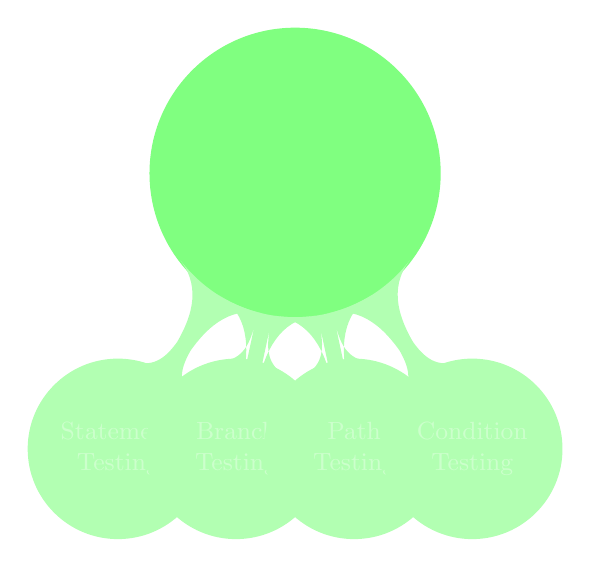
\begin{tikzpicture}[
    mindmap,
    concept color=green!30,
    every node/.style={concept, execute at begin node=\hskip0pt},
    root concept/.append style={concept, color=green!50, minimum size=3cm, font=\bfseries},
    level 1 concept/.append style={level distance=3.5cm, sibling angle=90, color=green!20}
]
    \node [root concept] {White Box\\Testing}
        child { node {Statement\\Testing} }
        child { node {Branch\\Testing} }
        child { node {Path\\Testing} }
        child { node {Condition\\Testing} };
\end{tikzpicture}
\captionof{figure}{White Box Testing Techniques}
\end{center}

\begin{itemize}
    \item \keyword{Coverage Analysis}: Measures effectiveness of testing (e.g., statements executed / total statements)
    \item \keyword{Advantages}: Thorough testing, identifies dead code, ensures quality
    \item \keyword{Disadvantages}: Requires code knowledge, time-consuming
\end{itemize}
\end{solutionbox}

\begin{mnemonicbox}
\mnemonic{White Box Sees Inside Code Structure: Core concept.}
\end{mnemonicbox}

\end{document}
